


% \begin{figure}[tb!]
%   \centering
%   % \figfont{A}\hspace{3.2in}\figfont{B}\\
%   \includegraphics[width=\textwidth]{./gfx/All25GAPerf-Mean-Stretch.eps}
%   \caption{Mean and best performing genome of the GA population across
%     generations is shown for 3 simulations fro ech cost function. The
%     mark to the right of each graph is the 95 percentile range of the
%     target genome.}\label{fig:All25GAPerfLog}
% \end{figure}



\begin{figure}[tb!]
  \centering
  % \figfont{A}\hspace{3.2in}\figfont{B}\\
  \includegraphics[width=\textwidth]{./gfx/best25b.eps}
  \caption{Cross comparison of best genomes generated using GA with 25
    repetitions, measured against the target, 1-unit and 5-unit parameter
    perturbation distributions.  The bars show the mean of all three best
    genomes evaluated ten times for each cost function (error bars 2*stdev). For
    reference, horizontal lines show the median of the distribution of
    parameter perturbation for 1-step (dark line) and 5-steps (light
    line). {\textbf{Error bars are still sd not standard error.}}}\label{fig:R2}
\end{figure}


\newpage



% \begin{tabularx}{0.95\textwidth}{X|c|c}
%   Simulation                & MeanPE  & Score   \\\hline
%   stdyn diffAN sim1 min ga  & 22.1167 & 	10.1671 \\ 
%   stdyn diffAN sim2 min ga  & 31.6833 & 	10.0115 \\ 
%   stdyn diffAN sim3 min ga  & 12.7833 & 	9.67888 \\ \hline 
%   ifrga25 diffAN sim1 min ga& 22.2833 & 	0.238577 \\ 
%   ifrga25 diffAN sim2 min ga& 25.3167 & 	0.236389 \\ 
%   ifrga25 diffAN sim3 min ga& 28.5167 & 	0.23757 \\ \hline
%   ivga25 diffAN sim1 min ga & 26.2833 & 	0.216678 \\ 
%   ivga25 diffAN sim2 min ga &  25.45  & 0.207727 \\ 
%   ivga25 diffAN sim3 min ga & 29.3833 & 	0.21564 \\\hline
% \end{tabularx}

\clearpage

\begin{figure}[tb!]
  \centering
  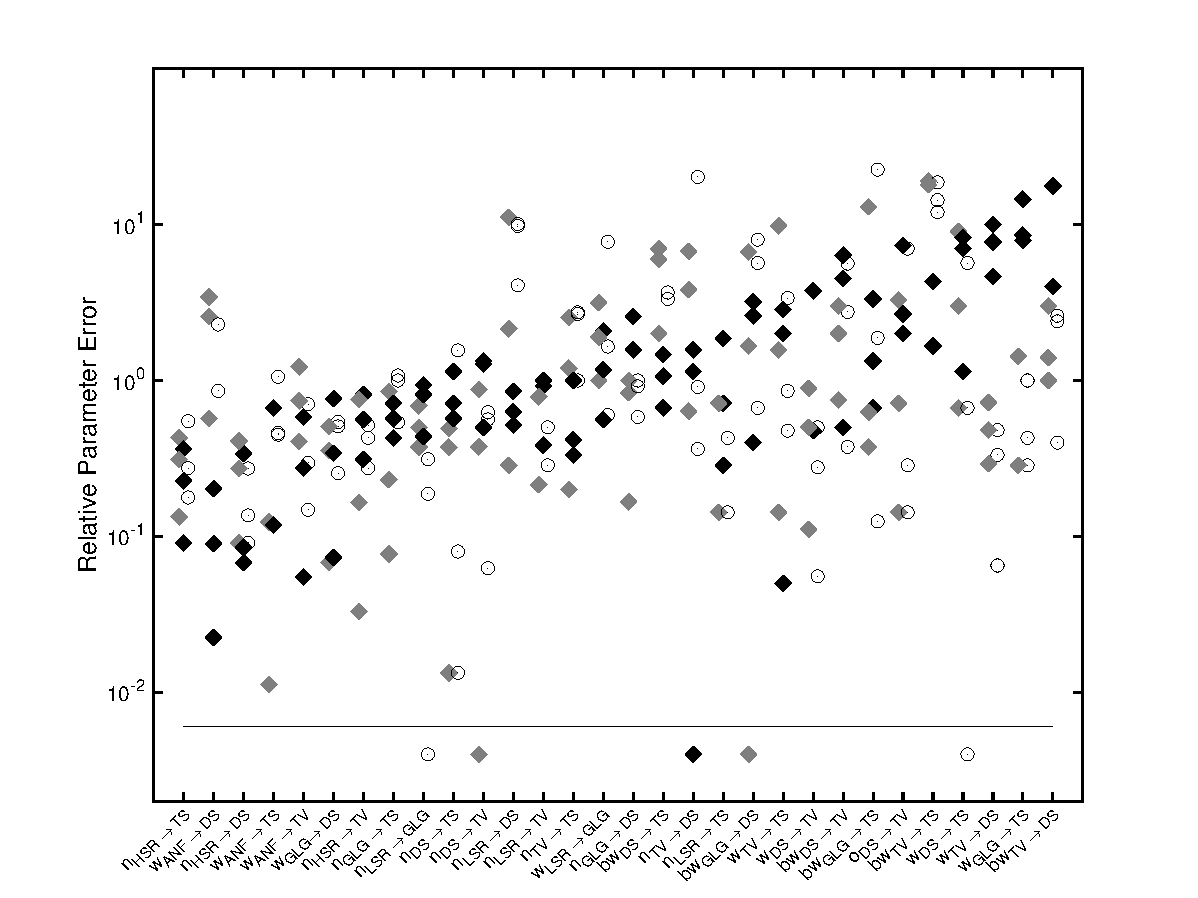
\includegraphics[width=\textwidth]{BestGenomesReRaw_CombinedLog.eps}
  \caption{Parameter errors of the best genomes in 3 GA
    simulations for each cost function: ST (${\color{halfgray} \diamond }$), IFR (${\color{black} \diamond }$), and AIV (${\circ}$). Errors were normalised in terms
    of the target parameter values ( (target - bestgenome)/target )}\label{fig:R2b}
\end{figure}


% \begin{tabularx}{0.95\textwidth}{X|c|c}
%   Simulation                &  Mean PE  & Score   \\\hline
%   stdyn diffAN sim1 min ga  & 	2.717	& 10.1671\\
%   stdyn diffAN sim2 min ga  & 	2.65462	& 10.0115\\
%   stdyn diffAN sim3 min ga  & 	1.14567	& 9.67888\\
%   ifrga25 diffAN sim1 min ga & 	2.05747	& 0.238577\\
%   ifrga25 diffAN sim2 min ga & 	1.88977	& 0.236389\\
%   ifrga25 diffAN sim3 min ga & 	2.30701	& 0.23757\\
%   ivga25 diffAN sim1 min ga & 	1.75237	& 0.216678\\
%   ivga25 diffAN sim2 min ga & 	2.40766	& 0.207727\\
%   ivga25 diffAN sim3 min ga & 	3.01355	& 0.21564\\\hline
% \end{tabularx}

% \begin{tabularx}{0.95\textwidth}{X|c|c}
%   Simulation         &  Mean PE  & Score   \\\hline
%   stdyn100 diffAN min ga	  & 1.97726	& 7.86038\\ \hline
%   ifr100 diffAN min ga	  & 2.1697	& 0.154698\\
%   ivga100 diffAN min ga	  & 2.32565	& 0.0292369 \\
% \end{tabularx}



\newpage


\begin{figure}[tb!]
  \centering
  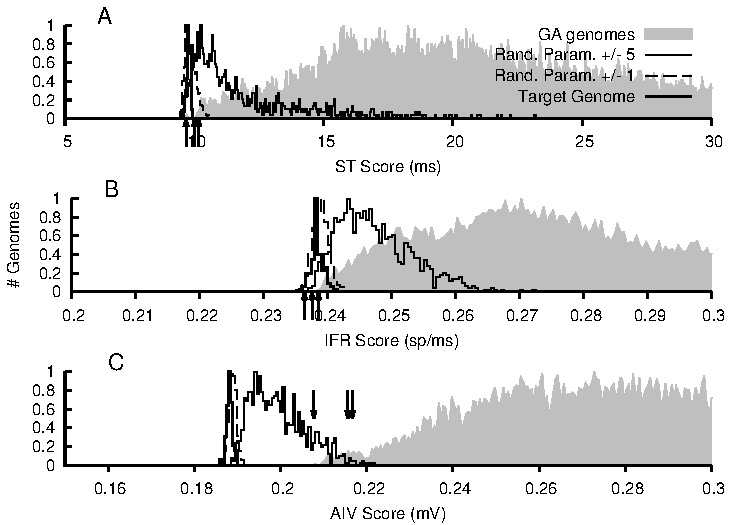
\includegraphics[width=\textwidth]{Histograms-Normalised.eps}  
  \caption{Histograms of simultaneous parameter perturbation of each cost
    function. The distribution of genomes in gray are all genomes evaluated by
    the GA that obtained the lowest score. The best scores of 3 GA simulations
    are pointed to by the arrows. The histograms show the distributions of 100
    target genome scores (thick line), 1000 genomes deviated by 1 unit step away
    from the target value (dashed line), and 1000 genomes deviated by 5 steps
    (thin line) from the target. The input spike generation and network
    connections for each parameter set (genome) were randomly generated for each
    evaluation.  All graphs are normalised to the peak value in each
    histogram.\label{fig:R3}}
\end{figure}

\clearpage


\begin{figure}[tb!]
  \centering
  % \figfont{A}\hspace{3.2in}\figfont{B}\\
  \includegraphics[width=\textwidth]{All100GAPerf.eps}
  \caption{Performance of the GAs best performing genome run with 100 repetitions.each
    generation is shown for each simulation. The mark to the right of
    each graph is the mean score and 95 percentile range of the target
    genome (error bars 2*sd).}\label{fig:R5}
\end{figure}
bigger target dots, blue lines in gray




% \section{FIG R6}
\begin{figure}[tb!]
  \centering
  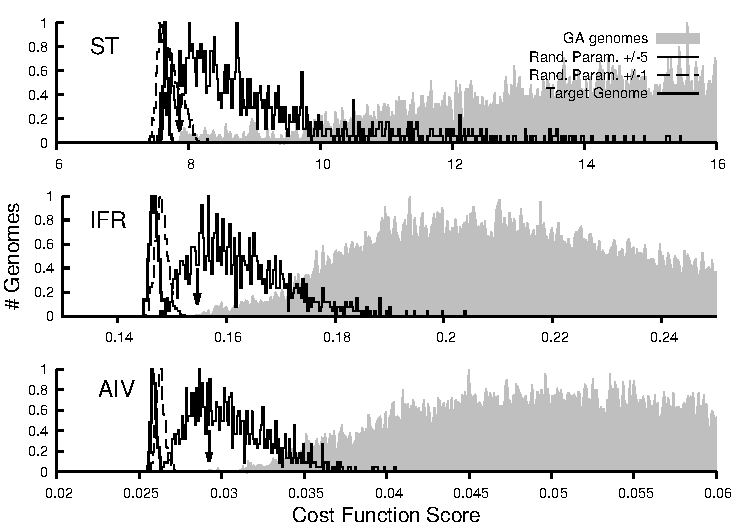
\includegraphics[width=\textwidth]{Histograms100-MaxNorm.eps}  
  \caption{Histograms of simultaneous parameter perturbation using 100 repetitions. All graphs are similar to
    Fig.~\ref{fig:R4}. % The
    % distribution of genomes evaluated during one GA are shown in gray
    % and the best scores of 3 simulation are pointed to by the
    % arrows. The histograms show the distributions of 100 target genome
    % scores (thick line), 1000 genomes deviated by 1 unit step away from
    % the target value (dashed line), and 1000 genomes deviated by 5 steps
    % (thin line) from the target. The input spike generation and network
    % connections for each parameter set (genome) were randomly generated
    % for each evaluation. 
  }\label{fig:R6}
\end{figure}
\clearpage




\begin{figure}[tb!]
  \centering
  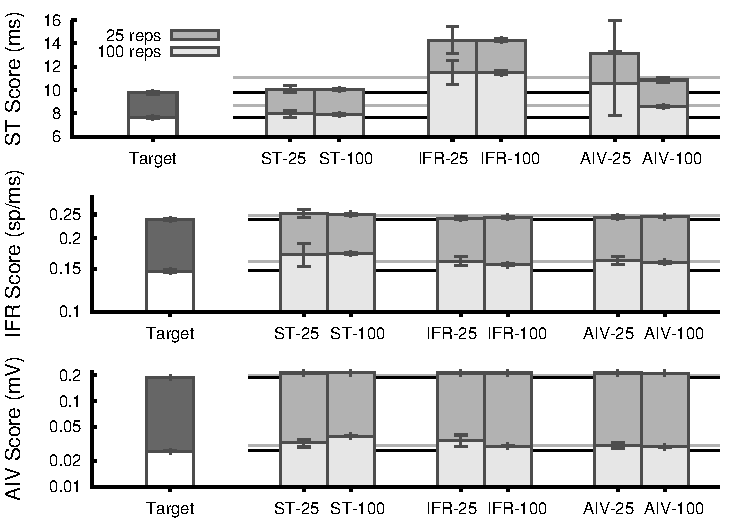
\includegraphics[width=\textwidth]{best25+100.eps}
  \caption{Comparison of Best genomes trained with different inputs using 100 or
    25 repetitions.  Target genome was run 100 times and each GA best genomes
    were run 10 times. For reference, horizontal lines show the the median of
    the distribution of parameter perturbation for 1-step (dark line) and
    5-steps (light line).}\label{fig:R7}
\end{figure}
